
\begin{figure}
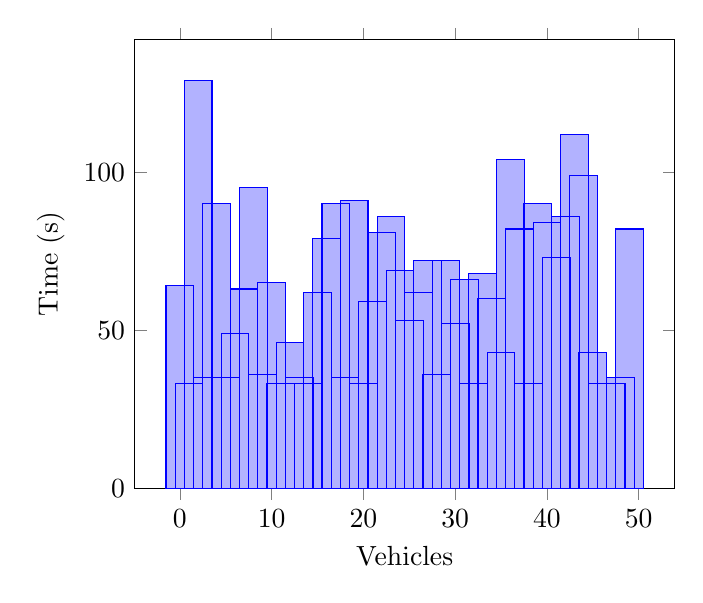
\begin{tikzpicture}
\begin{axis}[
legend style={anchor=west},
xlabel=Vehicles,
ylabel=Time (s),
ymin=0,
ybar,
]
\addplot coordinates {
(0, 64)
(1, 33)
(2, 129)
(3, 35)
(4, 90)
(5, 35)
(6, 49)
(7, 63)
(8, 95)
(9, 36)
(10, 65)
(11, 33)
(12, 46)
(13, 35)
(14, 33)
(15, 62)
(16, 79)
(17, 90)
(18, 35)
(19, 91)
(20, 33)
(21, 59)
(22, 81)
(23, 86)
(24, 69)
(25, 53)
(26, 62)
(27, 72)
(28, 36)
(29, 72)
(30, 52)
(31, 66)
(32, 33)
(33, 68)
(34, 60)
(35, 43)
(36, 104)
(37, 82)
(38, 33)
(39, 90)
(40, 84)
(41, 73)
(42, 86)
(43, 112)
(44, 99)
(45, 43)
(46, 33)
(47, 33)
(48, 35)
(49, 82)
};

\end{axis}
\end{tikzpicture}
\label{tik:100:18_N, 18_N.-60, 20_O, 21_O}
\caption{100 percent diving with GSC on route $18_N, 18_N.-60, 20_O, 21_O$}
\end{figure}
